\documentclass[11pt,a4paper]{article}
\usepackage[utf8]{inputenc}
\usepackage[portuguese]{babel}
\usepackage[T1]{fontenc}
\usepackage[left=1.7cm,right=1.5cm,top=2.5cm,bottom=2cm]{geometry}
\usepackage{xcolor}
\definecolor{orange}{RGB}{255,127,0}
%\usepackage[dvipsnames]{xcolor}
\usepackage{titlesec}
\usepackage[utf8]{inputenc}
\usepackage[portuguese]{babel}
\usepackage[T1]{fontenc}
\usepackage{amsmath}
\usepackage{amsthm}
\usepackage{amsfonts}
\usepackage{amssymb}
\usepackage{graphicx}
\usepackage{stackengine}
\usepackage{accents}
\usepackage{xcolor}
\usepackage{bbm}
\usepackage{enumitem}
\usepackage{mathtools}
\usepackage{ mathrsfs }
\newtheorem{teo}{\underline{Teorema}}
\newtheorem*{defi}{\underline{Definição}}
\newtheorem{prop}{\underline{Proposição}}
\newtheorem{prop2}{\underline{Propriedade}}
\newtheorem*{col}{\underline{Corolário}}
\newtheorem{lema}{\underline{Lema}}
\usepackage{bbm}
\newcommand{\e}{\mathbb{E}}
\newcommand{\var}{\mathrm{Var}}
\newcommand{\cov}{\mathrm{Cov}}
\newcommand{\p}{\mathbb{P}}
\newcommand{\dis}{\displaystyle}
\usepackage{subfigure}
\usepackage{hyperref}
\usepackage{listings}
\lstset{ %
  language=R, 					  % the language of the code
  backgroundcolor=\color{white},                  
  basicstyle=\footnotesize,       % the size of the fonts that are used for the code
  numbers=left,                   % where to put the line-numbers
  numberstyle=\tiny\color{black},  % the style that is used for the line-numbers
  stepnumber=1,                   % the step between two line-numbers. If it's 1, each line
                                  % will be numbered
  numbersep=5pt,                  % how far the line-numbers are from the code
  backgroundcolor=\color{white},  % choose the background color. You must add \usepackage{color}
  showspaces=false,               % show spaces adding particular underscores
  showstringspaces=false,         % underline spaces within strings
  showtabs=false,                 % show tabs within strings adding particular underscores
  frame=single,                   % adds a frame around the code
  rulecolor=\color{red},        % if not set, the frame-color may be changed on line-breaks within not-black text (e.g. commens (green here))
  tabsize=2,                      % sets default tabsize to 2 spaces
  captionpos=b,                   % sets the caption-position to bottom
  breaklines=true,                % sets automatic line breaking
  breakatwhitespace=false,        % sets if automatic breaks should only happen at whitespace
  title=   ,                 % show the filename of files included with \lstinputlisting;
                                  % also try caption instead of title
  keywordstyle=\color{black},      % keyword style
  commentstyle=\color{blue},   % comment style
  stringstyle=\color{black},      % string literal style
  escapeinside={\%*}{*)},         % if you want to add a comment within your code
  morekeywords={*,...}            % if you want to add more keywords to the set
}
\title{Atividade 3}
\author{Gabriel Mizuno}
\begin{document}
\maketitle

\section*{Funções Auxiliares}
Vamos usar 2 funções auxiliares para a realização dessa atividade.
\lstinputlisting[language=R]{FuncoesAuxiliares.R}

\section{Item a}[Usando Função Indicadora] \\
Vamos definir a seguinte v.a indicadora;$$I=\begin{cases} 1, & \mbox{se } \displaystyle\sum_{i=1}^5 iX_{i}\geqslant21.6\\ 0, & \mbox{caso contrario}\end{cases}$$  
Definindo $I$ dessa forma temos que:
$$\theta=\mathbb{E}[I]=\mathbb{P}\left( \displaystyle\sum_{i=1}^5 iX_{i}\geqslant21.6\right) $$.
\newpage
\lstinputlisting[language=R]{itema.R}

Vamos achar $\mathbb{E}[I]$ e assim estimar a probabilidade pedida
\lstinputlisting[language=R]{itema1.R}

E assim vamos achar $$\theta=0.175 $$
\section{Item b}[Variáveis Antagónicas]
\lstinputlisting[language=R]{itemb.R}
E assim vamos achar $$\theta=0.1708 $$
\newpage
\section{Item c}[Variável Controle]\\
Definindo a variável controle $Z=\displaystyle\sum_{i=1}^5 iX_{i} \Rightarrow \mathbb{E}[Z]=15$ e $Var[Z]=55$.
Simulando $Cov(Y,Z)$, onde $Y=I$

\lstinputlisting[language=R]{itemc.R}

Vamos achar $\mathbb{E}[I]$ e assim estimar a probabilidade pedida
\lstinputlisting[language=R]{itemc1.R}

E assim vamos achar $$\theta=0.178 $$
\section{Item d}[Conclusão]\\
Codigo usado para comparar os resultados dos itens b e c.
\lstinputlisting[language=R]{itemd.R}

O gráfico se encontra na próxima pagina

\begin{center}
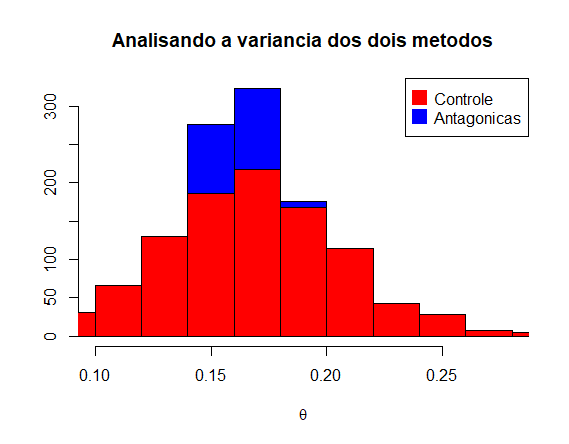
\includegraphics[width=.5\linewidth]{Grafico.png}
\end{center}

Portanto, concluímos que o método \textcolor{red}{Variável Controle} possui variância menor do que o método  \textcolor{blue}{Variáveis Antagónicas}, sendo assim escolheríamos o método   \textcolor{red}{Variável Controle} pois nesse método teríamos um estimado que em media acerta e teria um variância menor.

\end{document}